\documentclass[letterpaper,10pt]{article}
\usepackage{graphicx}
\usepackage[margin=2cm]{geometry}
\usepackage{url}
\usepackage{listings}

\title{Guided Programming: Consumers, Multiple Channels, and Sliding Windows}
\author{44-671: Streaming Data}
\date{}

\begin{document}
\maketitle

The same warnings that applied to notebooks and the Docker application from earlier assignments applies here.

When running a barbeque smoker, an accomplished (or even novice) pitmaster will closely monitor the temperatures of the cooking implement and the food to ensure everything is tasty.
Often on long cooks, the following (less than favorable) events can happen:
\begin{itemize}
	\item The temperature of the smoker can suddenly drop.
	\item The food hits a temperature where it is attempting to evaporate moisture, and it stays close to this temperature for an extended period of time (much like humans sweat to regulate temperature).  We call this the ``stall''.
\end{itemize}

Modern technology has graced us with thermometers that allow us to track and record temperatures and keep a history of the temperatures of both the smoker and the food over time.
We will be working with a data set generated from a thermometer that records the temperature \emph{every thirty seconds}.
The particular meal involved two different channels of data for food and the temperature of the smoker.
We will be looking at sliding windows of data to detect the events described above.
Specifically:
\begin{itemize}
	\item If the temperature of the smoker drops more than 15 degrees in 2.5 minutes, we want to alert the pitmaster that the smoker needs attention
	\item If the temperature of the food does not change by more than one degree over a 15 minute time period, we want to report that the food has hit the stall
\end{itemize}

The producer code that reads the historical data has been provided.

\begin{enumerate}
	\item Start your Docker application you set up in the Software Installation assignment
	\item Open a web browser and open JupyterLab (\url{http://localhost:8888/lab})
	\item Upload the following files:
		\begin{itemize}
			\item \texttt{bbq-producer.ipynb}
			\item \texttt{smoker-temps.csv}
		\end{itemize}
	\item Change the appropriate line in the producer notebook with your RabbitMQ Docker instance name
	\item Create a new Python Notebook named \texttt{yourname-consumer.ipynb} (replace \texttt{yourname} with your name)
	\item Create a new cell in your consumer notebook that contains the following code (make sure to change the name of the RabbitMQ Docker instance!):
		\begin{center}
			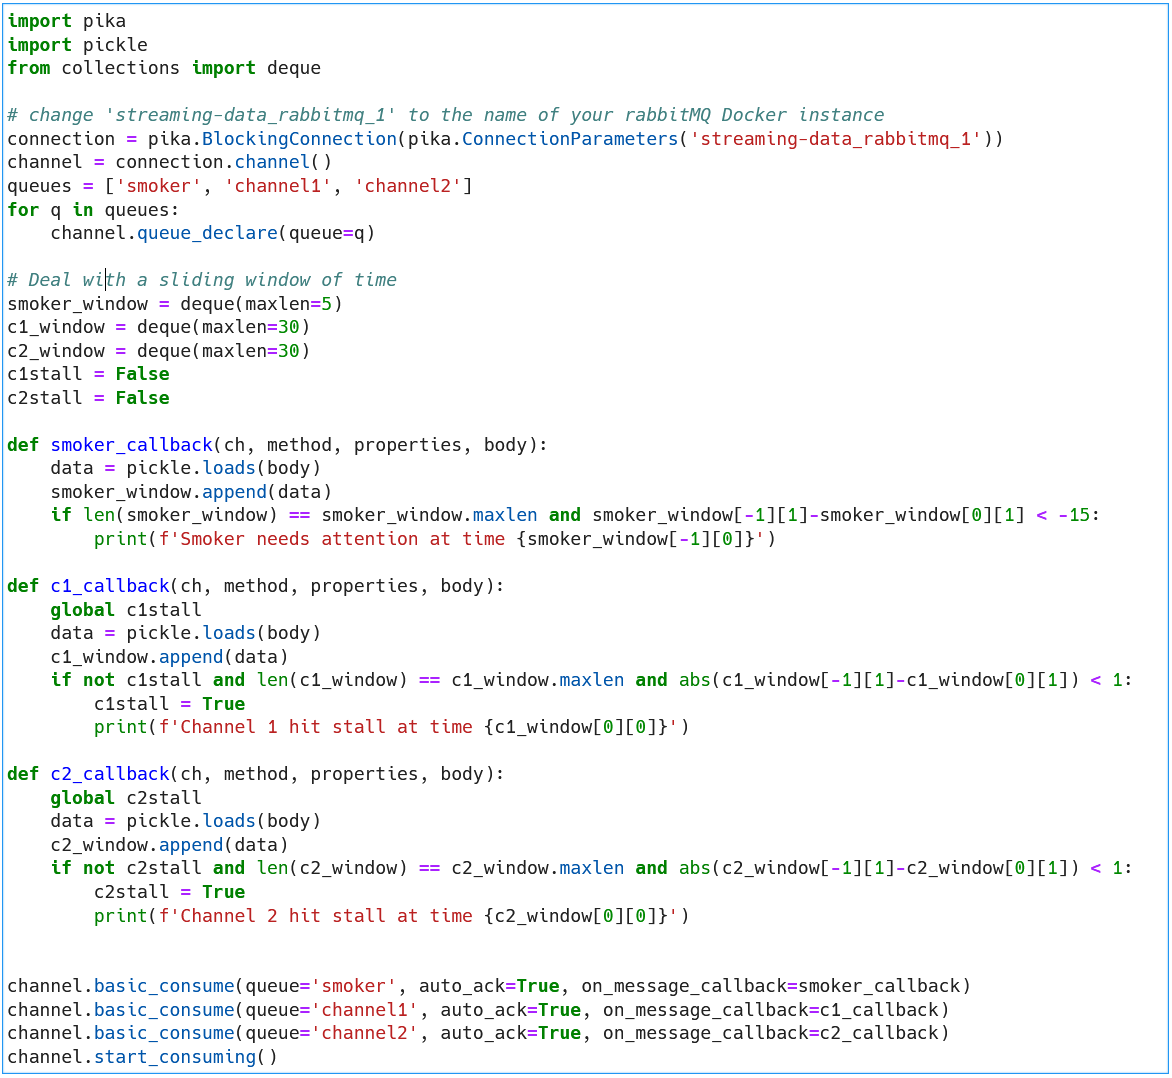
\includegraphics[width=0.9\textwidth]{consumer-code.PNG}
		\end{center}
	\item Create another cell in your consumer notebook with the code \texttt{connection.close()}
	\item Run your consumer code (the first cell you created); fix errors that occur!
	\item Run the producer code in the producer notebook
	\item Add a new Markdown cell at the bottom of your producer notebook and answer the following questions:
		\begin{itemize}
			\item What times did the smoker need attention?
			\item What time did channel 1 hit its stall? Channel 2?
			\item We used a sliding window approach; based on your reading of the Python Documentation (linked on the course website) how do you think we limited our code to only look at the last 2.5 minutes of smoker data and the last 15 minutes of food data?
			\item Why do you think a sliding window approach was more appropriate than other windowing approaches (or considering the entire temperature history)?  Do you think a different approach might be even better?  
			\item Why do you think we used different work queues for each channel of data?
		\end{itemize}
	\item ``Run'' your Markdown cell
	\item Export your notebook as a PDF (make sure it contains your answers and the output from your code!) and submit the PDF to the course website.
	\item Close your notebooks and stop Docker application; note there's no need to stop the producer (it knows when it is done generating data and stops itself).
\end{enumerate}
\end{document}
